% =============================================================================
% Energy-Localized Vericoding for Verus
% Apart x Atlas Secure Program Synthesis Hackathon, May 2026 (Track 3)
% =============================================================================
\PassOptionsToPackage{unicode}{hyperref}
\PassOptionsToPackage{hyphens}{url}
\documentclass[10pt]{article}

\usepackage{xcolor}
\usepackage{amsmath,amssymb,amsthm}
\usepackage{iftex}
\ifPDFTeX
  \usepackage[T1]{fontenc}
  \usepackage[utf8]{inputenc}
  \usepackage{textcomp}
\fi
\usepackage{lmodern}
\usepackage{microtype}
\usepackage[margin=1in]{geometry}
\usepackage{parskip}
\usepackage{booktabs}
\usepackage{multirow}
\usepackage{graphicx}
\graphicspath{{.}{figures/}}
\usepackage{caption}
\usepackage{subcaption}
\usepackage{listings}
\usepackage{enumitem}
\usepackage{hyperref}
\usepackage{cleveref}
\hypersetup{
  colorlinks=true,
  linkcolor=black,
  citecolor=blue!50!black,
  urlcolor=blue!50!black,
  pdfcreator={LaTeX}
}
\setlength{\emergencystretch}{3em}

% Code listing style for Verus snippets.
\lstdefinelanguage{Verus}{
  basicstyle=\ttfamily\small,
  keywords={fn,let,mut,if,else,while,for,return,struct,enum,impl,trait,pub,use,as,in,match,move,ref,Self,self},
  morekeywords=[2]{requires,ensures,invariant,decreases,assert,assume,exists,forall,spec,proof,exec,verus,broadcast,old,recommends},
  keywordstyle=\color{blue!60!black}\bfseries,
  keywordstyle=[2]\color{purple!60!black}\bfseries,
  commentstyle=\color{gray!70!black}\itshape,
  morecomment=[l]{//},
  stringstyle=\color{green!50!black},
  showstringspaces=false,
  breaklines=true,
  frame=single,
  framerule=0.2pt,
  rulecolor=\color{gray!50},
  numbers=left,
  numberstyle=\tiny\color{gray},
  numbersep=8pt,
  xleftmargin=20pt,
  framexleftmargin=15pt,
}
\lstset{language=Verus}

\title{\textbf{Where to Look:\\
  Energy-Based Fault Localization for Verus Vericoding}}
\author{Guy Nachshon \\ \small Oz Labs \\ \small \texttt{guy@ozlabs.ai}}
\date{Apart $\times$ Atlas Computing $\cdot$ Secure Program Synthesis Hackathon, May 2026}

\begin{document}
\maketitle

% =============================================================================
\begin{abstract}
We study per-line fault localization for Verus, the Rust-based
verified programming language. Our model is a Qwen2.5-Coder-1.5B
LoRA specialist with sentinel tokens, per-line scalar energies, and
a scalar attention-pool head trained on broken/fixed sibling pairs
from the Microsoft Verus Training Data. On a marker-stripped corpus
of $609$ hand-authored failing Verus tests scraped from
\texttt{verus-lang/verus}, the final scalar-head hybrid reaches
AUROC $=0.78$, top-1 $=0.56$, and top-3 $=0.84$. It beats six static
baselines, but is matched or beaten by five zero-shot frontier LLMs
on per-line ranking, pass/fail discrimination, and closed-loop CEGIS
repair with the Verus toolchain in the loop. The contribution is
therefore calibration rather than specialist superiority: we release
the small-model baseline, line-labeled corpus, LLM and CEGIS
records, and a strip-FAILS audit pipeline that exposed a
\texttt{// FAILS}/\texttt{// FIXME} marker leak in an earlier
checkpoint.
\end{abstract}

% =============================================================================
\section{Introduction}
\label{sec:intro}

Verified languages such as Verus~\cite{verus2023} attach formal
specifications to Rust-like code and discharge proof obligations to
an SMT solver. Recent vericoding work shows that LLMs can draft
Verus from natural-language specs and refine it from verifier
feedback~\cite{verus_training_data}. When a draft fails, a useful
next signal is \emph{where} to repair: a localizer could focus a
CEGIS-style~\cite{cegis} repair loop on the top-$k$ suspicious lines
instead of resampling the whole implementation.

We cast this as discriminative energy-based modeling in the LeCun
sense~\cite{lecun2006tutorial}. Given a spec and implementation, the
model emits an unnormalized scalar energy for each scorable line and
is trained from broken/fixed sibling structure in the Microsoft Verus
Training Data. The final system is small enough to fine-tune with
LoRA on one A100, yet produces a differentiable line-level suspicion
field and a separately trained scalar head for whole-implementation
ranking.

The central empirical story is mixed. The model is a strong static
baseline, but frontier LLMs remain stronger, and our CEGIS experiment
finds no repair-rate advantage. The audit story is equally important:
an earlier checkpoint looked much better until a strip-FAILS audit
showed that Qwen's pretrained comment-token priors were leaking
through \texttt{// FAILS}/\texttt{// FIXME} markers.

\paragraph{Contributions.}
\begin{enumerate}[leftmargin=*,itemsep=2pt,topsep=2pt]
\item \textbf{A discriminative energy-based per-line fault
  localizer for Verus.} The scalar-head hybrid (Qwen2.5-Coder-1.5B
  + LoRA + sentinel line energies) reaches AUROC $=0.78$, top-1
  $=0.56$, and top-3 $=0.84$ on the marker-stripped dev-test corpus
  ($n=1{,}492$). \Cref{sec:methods,sec:results:headline,sec:results:run10-baselines}.
\item \textbf{An architectural ablation isolating the load-bearing
  component.} Single-knob ablations attribute the $+30$pp AUROC gain
  over the adversarial-marker LSE design to the scalar attention-pool
  head; listwise loss and semi-hard mining help less, and
  logistic-vs-hinge is within noise (\Cref{app:marker-aug},
  \Cref{tab:run10-ablation}).
\item \textbf{A strip-FAILS audit pipeline.} We document a Qwen
  pretraining-prior leak that inflated an earlier checkpoint by
  $33$pp top-3, then show that our fix overshot into marker-aversion
  while frontier LLMs are nearly marker-invariant
  (\Cref{sec:results:llm-marker-audit,sec:results:strip-fails-audit}).
\item \textbf{Comprehensive evaluation against external baselines.}
  The model beats every static baseline, but frontier LLMs match or
  beat it on ranking, discrimination, and CEGIS repair
  (\Cref{sec:results:llm-zeroshot,sec:results:cegis}).
\end{enumerate}

\paragraph{Scope.} We evaluate per-line fault localization on
hand-authored Verus failing tests and a closed-loop CEGIS
repair-rate-at-$1$ experiment at $n=100$. Transfer to Dafny~\cite{dafny},
F\textsuperscript{*}, or other verifiers is not addressed. All model
numbers are from one training seed; bootstrap CIs capture corpus
sampling variance, not seed variance.

% =============================================================================
\section{Related Work}
\label{sec:related}

\paragraph{Process Reward Models (PRMs).}
PRMs score intermediate reasoning steps and aggregate them into an
outcome score~\cite{lightman2023letsverify,wang2024mathshepherd,setlur2024processadvantage,cobbe2021verifiers}.
Our setting is analogous, but the steps are Verus source lines and
the supervision comes from broken/fixed sibling pairs rather than
human labels or Monte Carlo rollouts. We also study the train/eval
aggregator mismatch (``assessment drift'') highlighted by
\cite{zhang2025lessonsprm}.

\paragraph{Energy-based models.}
We follow the discriminative EBM framework of
LeCun et al.~\cite{lecun2006tutorial}: unnormalized scalar energy,
contrastive training, and no generative sampling. Related recipes
include JEM-style classifier-EBMs~\cite{grathwohl2020jem},
compositional EBMs~\cite{du2019ebm}, and residual EBMs for
text~\cite{bakhtin2021residual}.

\paragraph{Fault localization.}
Spectrum-Based Fault Localization~\cite{abreu2007ochiai} (Ochiai, Tarantula,
DStar) ranks lines by their differential presence in failing vs.\ passing
runs. We adapt Ochiai to broken/fixed siblings as an oracle-style
structural baseline; at deployment no PASS sibling exists, so it is
not a deployable localizer.

\paragraph{Mutator validity.}
Just et al.~\cite{just2014mutants} and Pradel and Sen~\cite{pradel2018deepbugs}
show that mutator-trained bug detectors can degrade sharply on real
defects; Allamanis et al.~\cite{allamanis2021ssbd} report similar
gaps for self-supervised detectors. We therefore evaluate on
hand-authored Verus failures rather than only mutator-generated held
sets (\Cref{sec:methods:real-bug}).

% =============================================================================
\section{Methods}
\label{sec:methods}

\subsection{Problem setting and notation}
A spec--impl pair $(s, c)$ consists of the spec block $s$
(\texttt{requires}, \texttt{ensures}, \texttt{invariant}, \texttt{decreases}
clauses plus the \texttt{fn} signature) and an implementation body $c$ with
scorable lines $c_1, \dots, c_N$. Each $(s,c)$ has a binary outcome
$y \in \{\text{pass}, \text{fail}\}$ from running Verus on the concatenation.
For broken/fixed sibling pairs from \texttt{sft\_safe} we additionally have
$B \subset \{1,\dots,N\}$, the set of \emph{buggy line indices} obtained by
\texttt{difflib} comparison with the fixed sibling.

The model assigns to each line a scalar energy $E_\theta(c_i \mid s, c)$
(higher = more buggy), aggregates them via log-sum-exp at temperature $T$:
\begin{equation}
\label{eq:lse}
E_\theta(c \mid s) \;=\; T \cdot \log \left[ \tfrac{1}{N} \sum_{i=1}^{N}
\exp\!\left( E_\theta(c_i \mid s, c) / T \right) \right],
\end{equation}
which interpolates between mean ($T \to \infty$) and max ($T \to 0$) and is
mean-normalized so the aggregate does not scale with implementation length.

\subsection{Architecture}
\label{sec:methods:arch}
The backbone is Qwen2.5-Coder-1.5B~\cite{qwen25coder} with LoRA
adapters~\cite{hu2021lora} ($r{=}16$, $\alpha{=}32$) on all linear modules
and a rank-8 LoRA on \texttt{embed\_tokens}, $\sim$20M trainable parameters
out of 1.56B total. A sentinel token (\verb+<|fim_pad|>+, repurposed from
Qwen's FIM vocabulary) is inserted after each scorable impl source line; the
per-line head $\text{MLP}: \mathbb{R}^{1536} \to \mathbb{R}$
(two-layer with GELU, dropout 0.1, hidden 256) reads each sentinel's
final-layer hidden state and emits an unbounded scalar energy. The
sentinel's causal attention sees the spec and all preceding impl lines.

\paragraph{Backbone choice.}
We chose Qwen2.5-Coder-1.5B for reproducibility and engineering fit,
not because it was the newest or strongest code model available in
2026. Before training, we ran two tokenizer/license sweeps on a
canonical Verus snippet using actual tokenizer probes. In the first
sweep, Qwen2.5-Coder-1.5B/3B used 173 tokens and kept
\texttt{requires}, \texttt{ensures}, \texttt{invariant}, and
\texttt{decreases} as single tokens; StarCoder2-3B used 187 tokens,
DeepSeek-Coder-V2-Lite 205, ModernBERT-base 193, UniXcoder-base 194,
and CodeBERT-base 256. A broader second sweep found shorter
candidate tokenizations from OpenCoder-1.5B-Base (167 tokens) and
DeepSeek-Coder-6.7B-base (159 tokens), but the former required
additional license review and the latter changed the compute and
ablation budget. Qwen2.5-Coder-1.5B was therefore the stable primary:
Apache-2.0, compact on Verus syntax, and FIM-pretrained in the same
vocabulary we use for line sentinels. In particular, the technical
report trains file- and repository-level fill-in-the-middle objectives
with \verb+<|fim_prefix|>+, \verb+<|fim_middle|>+,
\verb+<|fim_suffix|>+, and \verb+<|fim_pad|>+ tokens; our sentinel is
therefore not a newly added delimiter but a pretrained position type
whose hidden state the backbone was already trained to make useful.
The model is also small enough for LoRA sweeps and checkpoint release,
and strong enough to test whether localization supervision teaches a
capability beyond frozen-backbone surprisal. We evaluate newer
frontier LLMs separately as external zero-shot baselines rather than
as trainable specialist backbones.

\subsection{Losses}
\label{sec:methods:losses}
We optimize $L = \lambda_{\text{spec}} L_{\text{spec}} + \lambda_{\text{line}} L_{\text{line}}$ with
$\lambda_{\text{spec}} = 3$, $\lambda_{\text{line}} = 1$.

\paragraph{Within-spec InfoNCE.}
For each spec with mixed-label impls, the passing impl is the positive and
failing siblings (plus an in-batch cross-spec FAIL pool) are negatives;
the contrast is on whole-impl energies via \Cref{eq:lse}:
\begin{equation}
L_{\text{spec}} = -\log \frac{\exp(-E_\theta(c^+ \mid s))}{\sum_j \exp(-E_\theta(c_j \mid s))}.
\end{equation}

\paragraph{Within-impl pairwise hinge.}
For each broken sibling with $|B| > 0$, we sample pairs $(i, i')$ with
$i \in B$ and $i' \notin B$ and penalize with margin $m=1$:
\begin{equation}
L_{\text{line}} = \mathbb{E}_{(i,i')} \max\!\left(0, m + E_\theta(c_{i'}) - E_\theta(c_i)\right).
\end{equation}

The two losses operate on disjoint subsets of the batch
(\texttt{system\_trajectory} triples for $L_{\text{spec}}$, \texttt{sft\_safe}
broken impls for $L_{\text{line}}$); the sampler enforces a minimum count of
each per batch to avoid collapse.

\paragraph{Why not verifier-cited lines?}
We deliberately do not use Verus diagnostic line numbers as buggy-line
labels. In verified-code failures, the diagnostic often cites the
\emph{consuming} assertion, postcondition, or invariant where the SMT
obligation fails, not necessarily the source line that introduced the
bad value or insufficient proof. In the trajectory files, FAIL rows also
lack complete verifier logs, making diagnostic-derived line labels both
noisy and incomplete. Line-level supervision therefore comes only from
broken/fixed sibling diffs in \texttt{sft\_safe}/\texttt{sft\_part2};
diagnostic text is not used as a line-label source.

\subsection{Data and split}
\label{sec:methods:data}
A preliminary dataset audit found that most public ``verified code''
corpora are curated positives, theorem-proving traces, or prompt-only
sets: the failing implementation attempts needed for contrastive
localization have usually been filtered out. We therefore use the only
public source we found with both mixed-label spec siblings and explicit
broken/fixed repairs: four files from
\texttt{microsoft/Verus\_Training\_Data}. The two trajectory files
(\texttt{system\_trajectory\_843} and
\texttt{algorithmic\_trajectory\_9040}) provide 281 + 6{,}402
unique-spec impls at mixed pass/fail labels; the two SFT files
(\texttt{sft\_safe\_25k} and \texttt{sft\_part2\_4557}) provide
$\approx$14k broken/fixed sibling pairs with \texttt{difflib}-derived
$B$. After parsing, filtering for $|B| \le 3$ on sft\_*, and tokenization to
4096-token context, the merged corpus contains 31{,}505 examples across
5{,}382 unique normalized-spec texts.

\paragraph{Spec-text-disjoint split.}
We hash spec text after whitespace normalization to derive a spec key, and
split spec keys randomly into 29{,}525 train / 1{,}980 held-out examples.
This is strictly stronger than splitting on the dataset's \texttt{spec\_id}
field: we found that \texttt{spec\_id}-based splits leak 79\% of held-out
spec content into train under different IDs, inflating AUROC to 0.98 by
memorization. We assert post-split disjointness on normalized-text hashes.

\subsection{Real-bug evaluation corpus}
\label{sec:methods:real-bug}
To test transfer beyond the mutator distribution, we constructed a Verus dev-test
corpus from \texttt{verus-lang/verus} at HEAD. The repository's test suite
(\texttt{source/rust\_verify\_test/tests/*.rs}, 132 files) contains
hand-authored test cases bracketed by
\texttt{test\_verify\_one\_file! \{ ... \}} macros and paired with explicit
outcomes (\texttt{=> Ok(())} or \texttt{=> Err(...)}). Failing tests are
annotated by Verus developers with \texttt{// FAILS} comments on the exact
line that fails to verify---providing line-level ground truth that is
\emph{not} mutator-derived.

Parsing yields \textbf{1{,}492 records (609 FAIL with \texttt{// FAILS}
labels)} across 132 test files. Mean impl length 19 lines, matching
sft\_safe's 19.7 (no length-distribution confound). \textbf{We refer to
this set throughout as the ``Verus dev-test corpus.''} The bugs are
hand-authored failing test cases written by Verus contributors, not
production defects extracted from project bug reports; following
\cite{just2014mutants} we avoid calling them ``real bugs'' to prevent
confusion with the production-defect literature. They are nevertheless
a substantially harder transfer target than mutator-induced failures
(the model has never seen \texttt{verus-lang/verus} test sources during
training), and to our knowledge this is the largest publicly available
line-labeled Verus failure corpus --- larger than the $\sim$50-bug
Defects4J reference set used in earlier line-localization
work~\cite{just2014mutants}, though the two are not strictly comparable
(Defects4J indexes production Java defects across multiple repositories;
ours is hand-authored failing tests from a single repository).

% =============================================================================
\section{Results}
\label{sec:results}

\subsection{Specialist performance on the marker-stripped Verus dev-test corpus (scalar-head hybrid)}
\label{sec:results:headline}

The scalar-head hybrid (artifact run \#10), our final architecture, achieves
\textbf{AUROC $= 0.78$, top-1 $= 0.56$, top-3 $= 0.84$} on $n=1{,}492$
records ($609$ FAIL with labels) of the marker-stripped Verus
dev-test corpus. Baselines are in \Cref{sec:results:run10-baselines};
significance tests are in \Cref{tab:significance}. An earlier
checkpoint appeared to reach top-3 $=0.93$; \Cref{sec:results:strip-fails-audit}
explains why that number was marker-leaky.

\subsection{Scalar-head hybrid vs.\ static and learned baselines (canonical comparison)}
\label{sec:results:run10-baselines}

We compare against six execution-free baselines on the marker-stripped
dev-test corpus ($n=1{,}492$, $n_{\text{labeled}}=609$):

\begin{description}[leftmargin=1.5em,itemsep=0pt]
\item[\normalfont\textsc{Random}] Uniform $[0,1)$ per line; sanity floor.
\item[\normalfont\textsc{Length}] Rank longer lines higher.
\item[\normalfont\textsc{Verus keyword}] Count occurrences of Verus DSL
  annotations: \texttt{assert}, \texttt{ensures}, \texttt{invariant},
  \texttt{decreases}, \texttt{requires}, \texttt{forall}, \texttt{exists}, and
  \texttt{assume}.
\item[\normalfont\textsc{Marker keyword}] Count occurrences of authorial bug
  markers: \texttt{// FAILS}, \texttt{panic!}, \texttt{unwrap},
  \texttt{// TODO}, \texttt{assert!}, \texttt{todo!},
  \texttt{unimplemented!}, \texttt{unsafe}, and \texttt{// FIXME}; this is the
  leak-ceiling baseline.
\item[\normalfont\textsc{Diff-from-sibling}] Rank target lines by
  $1 - \max_{\text{PASS sib}} \mathrm{Jaccard}_{\text{bigram}}(\ell, \ell')$:
  a static adaptation of the NN-query baseline~\cite{renieris2003nnqueries}.
\item[\normalfont\textsc{Qwen surprisal}] Per-line average negative log-likelihood
  under the same Qwen2.5-Coder-1.5B backbone, frozen (no LoRA, no head).
  This is the code-naturalness floor~\cite{hindle2012naturalness,karampatsis2020openvocab}
  and the most direct test of whether fine-tuning helps.
\end{description}

\Cref{fig:baseline-comparison,fig:roc-curves,fig:topk-curves} summarize the
comparison; \Cref{tab:significance} gives paired McNemar and DeLong tests.

\begin{figure}[t]
\centering
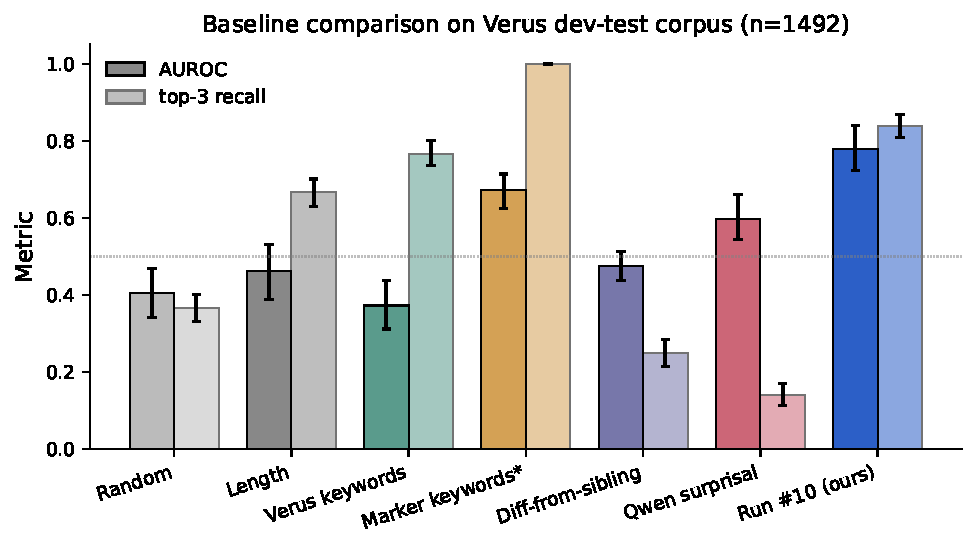
\includegraphics[width=0.95\linewidth]{fig_baseline_comparison.pdf}
\caption{Scalar-head hybrid vs six static baselines on the marker-stripped Verus dev-test
corpus ($n=1{,}492$). Bars: AUROC (solid) and top-3 recall (faded);
error bars are 95\% bootstrap CIs over 300 resamples. The marker-keyword
baseline (\normalfont\textsc{Marker keywords$^*$}) attains top-$3=1.00$ by design
(every record contains an authorial marker), but its impl-level AUROC of
$0.67$ is still substantially below the scalar-head hybrid's $0.78$ (DeLong
$p=0.006$). The scalar-head hybrid is the only method with both AUROC $>0.7$ and
top-$3>0.8$.}
\label{fig:baseline-comparison}
\end{figure}

\begin{figure}[t]
\centering
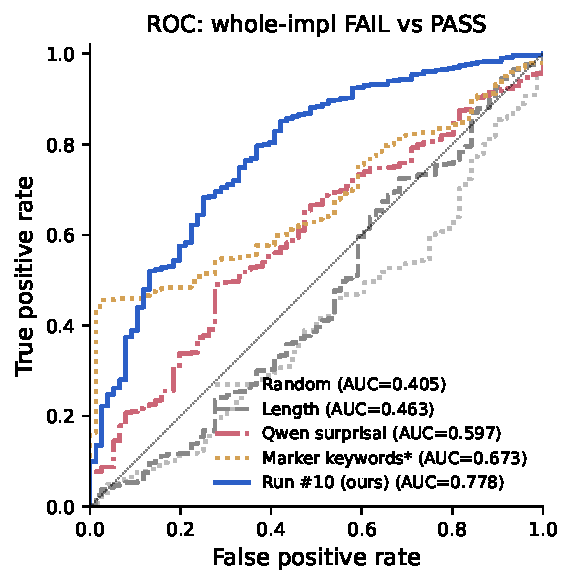
\includegraphics[width=0.55\linewidth]{fig_roc_curves.pdf}
\caption{ROC curves for whole-impl FAIL vs.\ PASS discrimination (scalar-head hybrid,
stripped, vs.\ four representative baselines). The scalar-head hybrid dominates
uniformly at every false-positive rate.}
\label{fig:roc-curves}
\end{figure}

\begin{figure}[t]
\centering
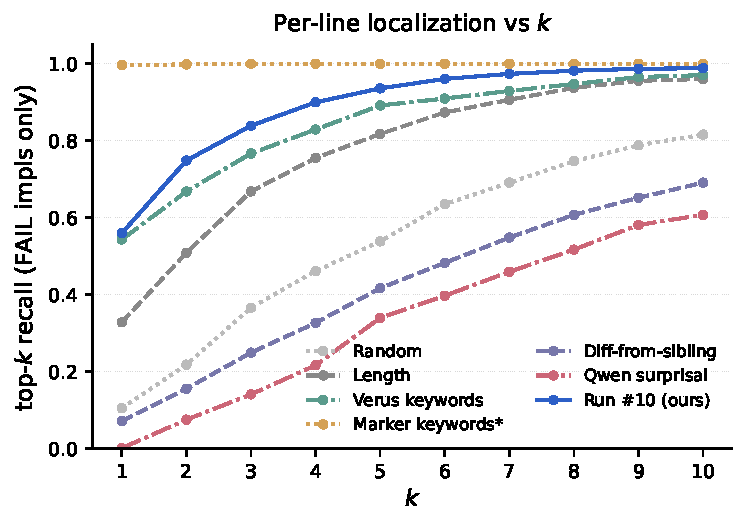
\includegraphics[width=0.75\linewidth]{fig_topk_curves.pdf}
\caption{Per-line localization recall as a function of $k$. The scalar-head hybrid reaches
top-$3=0.84$ where the strongest non-leak baseline (Verus keywords) needs
$k=5$ to match. The marker-keyword leak ceiling saturates at $1.00$ for all
$k\ge 1$ (and motivates the strip-FAILS audit).}
\label{fig:topk-curves}
\end{figure}

\paragraph{Headline finding.}
The scalar-head hybrid's AUROC of $0.78$ is $+18$pp over the frozen Qwen backbone
($0.60$; DeLong $p<10^{-5}$) and $+11$pp over the strongest non-leak
baseline (\normalfont\textsc{Marker keyword}, $0.67$; DeLong $p=0.006$). On per-line
top-$3$, the scalar-head hybrid ($0.84$) beats every non-leak baseline by $\ge +7$pp; the
margin over frozen Qwen surprisal is $+70$pp.

\paragraph{Honest reporting: top-$1$ vs.\ Verus keywords.}
The one place where the scalar-head hybrid's superiority is not statistically clean is
top-$1$ against \normalfont\textsc{Verus keyword} ($0.560$ vs.\ $0.544$, McNemar
$p=0.53$). Both rank assertion-like lines high. The gap becomes decisive at
top-$3$ ($p<10^{-4}$), top-$5$ ($p<10^{-2}$), and AUROC ($p<10^{-15}$).

\paragraph{Training dynamics.}
The impl-pair (scalar-head) loss collapses to near-zero within the
first $500$ steps, while the per-line listwise+pairwise loss keeps
improving through step $2{,}000$. Whole-implementation discrimination
is easier than localization in this setup.

\subsection{Comparison to frontier zero-shot LLMs}
\label{sec:results:llm-zeroshot}

We test five frontier LLMs via OpenRouter on the same marker-stripped
Verus dev-test subset used for the scalar-head hybrid ($n=220$:
$200$ FAIL $+ 20$ PASS, seed-fixed), with \emph{two} prompts:
(a) a \textbf{per-line ranking} prompt that asks for the top-$5$
most-suspicious line indices (\Cref{tab:llm-zeroshot}); (b) a
\textbf{discrimination} prompt that asks for $\{$pass, fail$\}$ plus
a calibrated $p(\text{fail})$ in $[0, 1]$
(\Cref{tab:llm-discrimination}, $n=250$: $200$ FAIL + $50$ PASS,
same FAIL subset). The LLMs see no \texttt{// FAILS} markers.

\textbf{Headline:} frontier zero-shot LLMs decisively outperform the
scalar-head hybrid on both ranking and discrimination.

\begin{table}[t]
\centering
\small
\caption{\textbf{Per-line ranking.} Frontier LLMs zero-shot vs.\
the scalar-head hybrid on the same $n=220$ subset of the marker-stripped Verus
dev-test corpus, ranking-prompt. \textbf{Bold} = best in column.
``Failures'' counts records where the model returned non-parseable
output.}
\label{tab:llm-zeroshot}
\begin{tabular}{lcccc}
\toprule
Method & top-1 & top-3 & top-5 & failures \\
\midrule
Random baseline                                 & 0.11           & 0.37           & 0.54           & ---                 \\
\textbf{Scalar-head hybrid (ours, 1.5B)}                  & 0.56           & 0.82           & 0.93           & ---                 \\
Claude Opus 4.7~\cite{anthropic2026claude47}    & 0.86           & 0.97           & 0.99           & 0 / 220             \\
GPT-5.5~\cite{openai2026gpt55}                  & 0.85           & 0.92           & 0.93           & 24 / 220            \\
Gemini 3.5 Flash~\cite{google2026gemini35}      & 0.89           & 0.98           & \textbf{1.00}  & 0 / 220             \\
Qwen 3.7 Max~\cite{qwen2026qwen37}              & \textbf{0.91}  & \textbf{0.99}  & 0.99           & 0 / 220             \\
DeepSeek V4 Pro~\cite{deepseek2026v4}           & 0.45           & 0.61           & 0.67           & 90 / 220 (41\%)$^\dagger$ \\
\bottomrule
\end{tabular}
\smallskip

{\footnotesize $^\dagger$ DeepSeek V4 Pro's $41\%$ parse-failure rate
is a budgeting artifact (its hidden chain-of-thought consumed the
1500-token output budget); we report the number for completeness but
note it is not a capability finding.}
\end{table}

\begin{table}[t]
\centering
\small
\caption{\textbf{Discrimination AUROC.} The same five LLMs prompted
with a $\{$pass, fail, $p(\text{fail}) \in [0,1]\}$ prompt on
$n=250$ records ($200$ FAIL + $50$ PASS, marker-stripped). AUROC is
computed over $p(\text{fail})$ against the true status; verdict
accuracy is exact-match against status. \textbf{Bold} = best in
column. Frontier zero-shot LLMs decisively outperform the scalar-head hybrid on
this metric too.}
\label{tab:llm-discrimination}
\begin{tabular}{lccc}
\toprule
Method & AUROC & verdict acc.\ & parse failures \\
\midrule
Random baseline                                 & 0.50           & ---            & --- \\
\textbf{Scalar-head hybrid (ours, 1.5B)}                  & 0.78           & ---            & --- \\
Claude Opus 4.7~\cite{anthropic2026claude47}    & 0.977          & 0.968          & 0 / 250 \\
Qwen 3.7 Max~\cite{qwen2026qwen37}              & 0.946          & 0.920          & 0 / 250 \\
Gemini 3.5 Flash~\cite{google2026gemini35}      & 0.983          & 0.956          & 0 / 250 \\
GPT-5.5~\cite{openai2026gpt55}                  & \textbf{0.984} & \textbf{0.981} & 38 / 250 \\
DeepSeek V4 Pro~\cite{deepseek2026v4}           & 0.914          & 0.914          & 64 / 250 \\
\bottomrule
\end{tabular}
\end{table}

\paragraph{Reading the result honestly.}
On per-line top-$k$, Claude, Qwen, and Gemini reach top-$3 \ge 0.97$
vs.\ the scalar-head hybrid's $0.82$, and top-$1 \ge 0.86$ vs.\ $0.56$.
On whole-impl AUROC, the gap is also large, though operationally less
important because the verifier itself supplies pass/fail with AUROC
$=1.0$. We use AUROC mainly as a sanity check that the scalar head
learned a coherent implementation-level signal.

\paragraph{What the table does \emph{not} establish.}
This comparison does not rule out specialist value under distribution
shift, API-cost constraints, self-judging-loop concerns, or future Verus
syntax. It does establish the negative calibration result on this corpus:
single-call frontier LLM localization is stronger.

\paragraph{Reproducibility note.}
Ranking-prompt model calls were made via OpenRouter on 2026-05-23
12:00--14:00 UTC; discrimination-prompt calls on 2026-05-23
22:55--23:25 UTC with explicit OpenRouter slugs and
$\text{temperature}=0$. Numbers may shift if providers update
snapshots; rerunnable scripts are
\path{scripts/baseline_llm_zeroshot.py} (ranking) and
\path{scripts/baseline_llm_discrimination.py} (discrimination).

\subsection{Marker-leak audit: invariance, reliance, and aversion}
\label{sec:results:llm-marker-audit}

The strip-FAILS audit asks how a localizer's top-$k$ ranking changes
when the \texttt{// FAILS} substring is removed at evaluation. We run
it on the same $n=220$ subset for the three strongest LLMs, on the
marker-leaky LSE checkpoint (run \#7, full corpus), and on the post-fix
scalar-head hybrid.

\begin{table}[t]
\centering
\small
\caption{Marker-leak audit, three regimes. ``With markers'' keeps
the \texttt{// FAILS} comment in the impl shown to the localizer;
``stripped'' removes it; $\Delta$ = with-minus-stripped, so
\emph{positive} $\Delta$ = marker-reliant (signal goes \emph{down}
when marker is removed), \emph{negative} $\Delta$ = marker-averse
(signal goes \emph{up} when marker is removed). LLM and scalar-head hybrid
numbers on the $n=220$ subset (same as \Cref{tab:llm-zeroshot});
marker-leaky LSE numbers on the full $n=1{,}492$ corpus where the leak
signal is largest (reproduced from \Cref{tab:strip-fails-headline}).}
\label{tab:llm-marker-audit}
\begin{tabular}{llccc}
\toprule
Model & Setting & top-1 & top-3 & top-5 \\
\midrule
\multicolumn{5}{l}{\textbf{Frontier LLMs (essentially marker-invariant)}} \\
Claude Opus 4.7    & with markers & 0.870    & 0.955          & 0.970 \\
                   & stripped     & 0.860    & 0.970          & 0.985 \\
                   & $\Delta$     & $+0.010$ & $-0.015$       & $-0.015$ \\[2pt]
Qwen 3.7 Max       & with markers & 0.920    & \textbf{1.000} & \textbf{1.000} \\
                   & stripped     & 0.905    & 0.985          & 0.985 \\
                   & $\Delta$     & $+0.015$ & $+0.015$       & $+0.015$ \\[2pt]
Gemini 3.5 Flash   & with markers & 0.925    & \textbf{1.000} & \textbf{1.000} \\
                   & stripped     & 0.890    & 0.980          & 1.000 \\
                   & $\Delta$     & $+0.035$ & $+0.020$       & $+0.000$ \\
\midrule
\multicolumn{5}{l}{\textbf{Marker-leaky LSE (artifact run \#7; marker-reliant)}} \\
Marker-leaky LSE (run \#7)     & with markers & 0.73     & 0.93           & 0.96  \\
                   & stripped     & 0.27     & 0.60           & 0.76  \\
                   & $\Delta$     & $+0.46$  & $+0.33$        & $+0.20$ \\
\midrule
\multicolumn{5}{l}{\textbf{Scalar-head hybrid (artifact run \#10; marker-averse)}} \\
Scalar-head hybrid & with markers & 0.055    & 0.265          & 0.535 \\
                   & stripped     & 0.560    & 0.815          & 0.930 \\
                   & $\Delta$     & $\mathbf{-0.505}$ & $\mathbf{-0.550}$ & $\mathbf{-0.395}$ \\
\bottomrule
\end{tabular}
\end{table}

\paragraph{Three regimes; the specialist never reaches invariance.}
Frontier LLMs are essentially marker-invariant ($|\Delta| \le 3.5$pp
top-1). The marker-leaky LSE checkpoint is marker-reliant: stripping
markers drops top-1 by 46pp. The scalar-head hybrid is marker-averse:
keeping markers drops top-1 by 50pp below its stripped performance,
to $0.055$, below the uniform-random floor. The adversarial marker
training broke reliance but overshot into anti-correlation.

\paragraph{What this means.}
The headline stripped numbers in \Cref{tab:run10-real-bug} are the
right deployment metric for marker-free inputs, but a leak-immune
localizer should sit near $\Delta=0$. Frontier LLMs do; both trained
specialists miss in opposite directions.

\subsection{Closed-loop CEGIS: does the specialist help \emph{repair}?}
\label{sec:results:cegis}

Static localization is only useful if it improves repair. We therefore
run a closed-loop CEGIS-style comparison, with the Verus toolchain
adjudicating success, analogous in spirit to fault-aware code editing
systems such as Self-Edit~\cite{zhang2023selfedit}.

\paragraph{Setup.} On $n=100$ tractable single-buggy-line FAIL
implementations ($\le 20$ scorable lines, $\le 25$ source lines), we
run three Claude Opus 4.7 repair arms and adjudicate each with
\texttt{verus} v0.2026.05.17:

\begin{description}[leftmargin=1.5em,itemsep=0pt]
\item[Arm A (specialist-guided):] Feed (spec, impl, the scalar-head hybrid's
  top-3 lines) to Claude Opus 4.7 with a ``rewrite the flagged
  lines to make Verus accept it'' prompt. Wrap the response,
  invoke Verus.
\item[Arm B (LLM-only resample):] Feed (spec, impl) to Claude
  with a ``rewrite the implementation to make Verus accept it''
  prompt --- no localization hint. Wrap, invoke Verus.
\item[Arm C (LLM-self-judged):] Two-pass Claude. First call:
  Claude ranks its own top-5 most-suspicious lines (same prompt
  as the ranking baseline in \Cref{tab:llm-zeroshot}). Second
  call: identical to Arm A but with Claude's own top-3 flagged
  instead of the specialist's. Wrap, invoke Verus.
\end{description}

Arm A tests specialist guidance, Arm B tests LLM-only resampling, and
Arm C tests whether Claude can supply its own localization hint.

\begin{table}[t]
\centering
\small
\caption{Closed-loop CEGIS repair-rate-at-1 on $n=100$ tractable
FAIL impls from the Verus dev-test corpus, adjudicated by the actual
Verus toolchain. Pairwise McNemar exact two-sided $p$-values on
discordant pairs; all three arms cluster at 25--30\% with no
statistically separable differences at $\alpha=0.05$.}
\label{tab:cegis-3arm}
\begin{tabular}{lc}
\toprule
Arm & Repair-rate-at-1 \\
\midrule
A. Specialist top-3 $\to$ Claude rewrite       & $0.25$ \\
B. LLM-only (Claude resample, no hint)         & $0.30$ \\
C. LLM-self-judged (Claude localize $\to$ rewrite) & $0.30$ \\
\midrule
\multicolumn{2}{l}{\emph{Pairwise discordance (only-A / only-other; McNemar $p$):}} \\
A vs.\ B  & 4 / 9, $p=0.27$ \\
A vs.\ C  & 0 / 5, $p=0.06$ \\
C vs.\ B  & 5 / 5, $p=1.00$ \\
\midrule
Union (any arm solved)        & $0.35$ \\
Intersection (all arms solved) & $0.21$ \\
\bottomrule
\end{tabular}
\end{table}

\paragraph{Honest reading.}
All three arms cluster at $25$--$30\%$ repair-rate, within each
other's 95\% bootstrap confidence intervals (roughly $\pm 9$pp).
\textbf{No arm is statistically separable at $\alpha=0.05$.} The point
estimates are directionally against the specialist, but the experiment
is underpowered; the $0$ specialist-only wins in A-vs-C disagreements
($p=0.06$) is a follow-up hypothesis, not a claim.

\paragraph{Structural finding.} The arms are not interchangeable. All
three solve $21$ impls, all three fail on $65$, and at least one arm
solves $35$. This leaves possible headroom for routing or ensembling,
but the $35\%$ union assumes an oracle router.

\paragraph{Methods footnote: Arm B prompt fix.} The initial Arm B
prompt omitted the failing impl and caused $38/100$ empty code blocks.
We reran Arm B with the failing impl as anchor, matching Arms A and C;
empty-block returns fell to $3$, and repair-rate moved from $0.27$ to
$0.30$. Both prompt versions are released in \texttt{artifacts/cegis/}.

\paragraph{What this means.}
On this corpus at this scale, specialist-guided repair does not
produce a detectable advantage over LLM-only or LLM-self-judged
repair. Per-line ranking, discrimination, and closed-loop repair all
point in the same direction.


\subsection{Whole-impl AUROC ceiling: an aggregator-invariance observation}
\label{sec:results:ceiling}

Whole-impl AUROC is sensitive to how line energies are aggregated. To
test whether the LSE head was simply the wrong reducer, we rescored the
same per-line outputs with standard permutation-invariant aggregators.
All remain near chance: mean, max, min, sum, last, and softplus-sum land
in $[0.47,0.53]$ (\Cref{tab:agg-sweep}). This supports the view that
bag-of-lines aggregation is the bottleneck for the LSE checkpoint.

For the scalar-head hybrid we report only the trained scalar
attention-pool head. Choosing a different reducer at evaluation time
would be assessment drift~\cite{zhang2025lessonsprm}; the sweep is a
diagnostic, not a headline metric.

\begin{table}[htbp]
\centering
\caption{Whole-impl AUROC on Verus dev-test corpus under different eval-time
aggregators of the \emph{same} per-line energies. All reducers cluster
around chance, supporting the information-theoretic ceiling argument.}
\label{tab:agg-sweep}
\small
\begin{tabular}{lc}
\toprule
Aggregator (eval-time, same per-line energies) & AUROC \\
\midrule
mean                       & 0.471 \\
max                        & 0.484 \\
min                        & 0.490 \\
last                       & 0.517 \\
sum                        & 0.530 \\
softplus-sum               & 0.475 \\
\midrule
\textbf{LSE (train-time matched)} & \textbf{0.487} \\
\bottomrule
\end{tabular}
\end{table}

\subsection{Statistical significance and subgroup analysis}
\label{sec:results:significance}

\paragraph{Significance vs.\ the length baseline.}
\Cref{tab:significance} reports paired McNemar tests for top-$k$ and
paired DeLong tests for AUROC. The audited scalar-head hybrid is
decisively better than length and frozen-Qwen baselines on top-$3$ and
AUROC, while top-$1$ against Verus-keyword is not significant. The
older pre-audit LSE-vs-length contingency is retained in the released
artifacts for historical comparability.

\paragraph{Bug-type breakdown.}
We bucket the Verus dev-test FAIL set by the syntactic context of the
\texttt{// FAILS}--annotated line (regex match on the line text):

\begin{table}[htbp]
\centering
\caption{Top-3 by lexical category of the \texttt{// FAILS}--annotated line on
the Verus dev-test corpus. Categories with $n \le 1$ omitted. \texttt{other}
denotes lines that do not lexically contain any of the listed Verus
keywords (typical content: variable assignments, arithmetic
expressions, method calls). \texttt{ensures} is the model's weakest
subgroup---a paper-worthy limitation discussed in
\Cref{sec:discussion}.}
\label{tab:bug-type}
\small
\begin{tabular}{lcc}
\toprule
Category at \texttt{// FAILS} line & $n$ & top-3 \\
\midrule
\texttt{assert}     & 369 & 0.943 \\
\texttt{other}      & 215 & 0.949 \\
\texttt{ensures}    & 22  & \textbf{0.591} \\
\bottomrule
\end{tabular}
\end{table}

The model is strong on \texttt{assert} and non-keyword lines, but
\texttt{ensures}-clause failures drop to top-3 $=0.59$ on $n=22$.

\paragraph{Why ensures-clauses are hard, mechanistically.}
The likely reason is architectural. A sentinel at line $\ell$ reads a
local causal hidden state, which works for assertions and arithmetic
whose signal is co-located with the line. Postcondition violations can
surface at an \texttt{ensures} line even when the causal explanation is
distributed upstream. A global-attention head alongside the local
sentinel head is the most direct follow-up.

\paragraph{Robustness across $|B|$ and impl length.}
We stratify the same Verus dev-test FAIL set two further ways:

\begin{table}[htbp]
\centering
\caption{Top-3 stratified by buggy-line count ($|B|$) and impl line-count
tertile, on the Verus dev-test corpus ($n=609$).}
\label{tab:strata}
\small
\begin{tabular}{lcc@{\hspace{2em}}lcc}
\toprule
$|B|$ stratum & $n$ & top-3 & Length stratum & $n$ & top-3 \\
\midrule
$|B|{=}1$  & 455 & 0.921 & short ($\le 8$ lines)   & 203 & \textbf{0.985} \\
$|B|{=}2$  & 73  & 0.973 & medium ($8$--$16$)      & 203 & 0.911 \\
$|B|{\ge}3$ & 81  & 0.951 & long ($16$--$139$)     & 203 & 0.897 \\
\bottomrule
\end{tabular}
\end{table}

Top-3 is robust across buggy-line count (no drop for hard $|B|=1$ vs.\
easier $|B|=2$). It degrades mildly with length, from $0.985$ on short
impls to $0.897$ on long ones.

\subsection{Strip-FAILS audit: where the pre-audit 0.93 number came from}
\label{sec:results:strip-fails-audit}
\label{sec:results:robustness}

The marker-leaky LSE checkpoint (run \#7) appeared to reach top-3
$=0.93$ on hand-authored Verus failures, suspiciously high for a model
trained on mutator data~\cite{just2014mutants,pradel2018deepbugs,allamanis2021ssbd}.
We audited this by re-scoring the same corpus after stripping
\texttt{// FAILS} comments at evaluation time.

\paragraph{The smoking gun: stripping markers collapses transfer.}
With markers retained, top-3 is $0.93$; stripped, it falls to $0.60$,
below the length baseline. The \texttt{// FAILS} substring carried a
large share of the apparent transfer.

\begin{table}[htbp]
\centering
\caption{Strip-FAILS audit on the Verus dev-test corpus
($n{=}1{,}492$, run \#7 step-500 checkpoint). The marker provides
substantial discriminative signal: top-3 falls $33$pp when markers are
stripped, dropping below the length baseline. We confirm the audit
generalizes by also stripping markers from baselines (which mostly do
not use them) and from the marker-keyword regex (which uses them by
construction --- bold row).}
\label{tab:strip-fails-headline}
\small
\begin{tabular}{lcc}
\toprule
                                & With \texttt{// FAILS}  & Stripped                \\
\midrule
top-1                           & 0.73                    & 0.27 ($-46$pp)          \\
\textbf{top-3 (marker-leaky LSE, run \#7)}  & \textbf{0.93}           & \textbf{0.60} ($-33$pp) \\
top-5                           & 0.96                    & 0.76 ($-20$pp)          \\
AUROC (LSE)                     & 0.49                    & 0.44                    \\
\midrule
Length baseline top-3           & 0.73                    & 0.46                    \\
Keyword baseline top-3          & 0.80                    & 0.55                    \\
\bottomrule
\end{tabular}
\end{table}

\paragraph{Mechanism: a Qwen pretraining-prior leak through the
\texttt{FAILS}/\texttt{FIXME} embeddings.}
The training corpus contains no \texttt{// FAILS} markers, so the LoRA
finetune had no reason to override Qwen's pretrained association between
tokens such as \texttt{FAILS}/\texttt{FIXME} and suspicious code.
Embedding-surgery confirms the mechanism (\Cref{app:marker-aug}); the
training-time mitigation is adversarial marker injection.

\paragraph{Alternative leak hypotheses.}
We ran targeted falsification tests for four alternatives.

\paragraph{No whole-text contamination.} Hash-based exact-match between
the Verus dev-test corpus and the full 31{,}505-example training set:
$\mathbf{0/1492}$ spec-text matches and $\mathbf{0/1492}$ impl-text
matches (whitespace-normalized).

\paragraph{Line-level leakage exists but does not drive the result.}
Some lines do recur: $39\%$ of scorable lines and $20.8\%$ of
comment-stripped buggy lines appear verbatim somewhere in training. But
the conditional test below shows overlap is not higher on hits.

\begin{table}[htbp]
\centering
\caption{Conditional train-overlap rate, split by whether the model's
top-1 prediction was correct on dev-test failures. If the model were winning
by memorization, HITs would show HIGHER train-overlap than MISSes.
The opposite holds.}
\label{tab:leak-conditional}
\small
\begin{tabular}{lcc}
\toprule
                                            & top-1 HIT ($n{=}445$) & top-1 MISS ($n{=}164$) \\
\midrule
pred-top1 in training corpus                & 20.9\%                & 27.4\%                  \\
ground-truth buggy line in training corpus  & 24.0\%                & 23.2\%                  \\
\bottomrule
\end{tabular}
\end{table}

This is the opposite of the memorization pattern.

\paragraph{Verus-keyword baseline.}
A DSL-aware baseline ranks by Verus keyword count. It is stronger than
length but does not explain the model's pre-audit top-$3$ result:

\begin{table}[htbp]
\centering
\caption{Verus-keyword baseline on both corpora, vs.\ length baseline
and our model. Keyword baseline beats length top-3 on both corpora,
but the model retains a $+17$pp (held) / $+13$pp (real) gap.}
\label{tab:keyword}
\small
\begin{tabular}{lcc}
\toprule
                            & Held top-3        & Dev-test top-3    \\
\midrule
Uniform random              & 0.40              & 0.38              \\
Length                      & 0.74              & 0.73              \\
Verus-keyword (this section)& 0.73              & 0.80              \\
\textbf{Ours (LSE)}         & \textbf{0.90}     & \textbf{0.93}     \\
gap vs.\ keyword            & $+17$pp           & $+13$pp           \\
\bottomrule
\end{tabular}
\end{table}

\paragraph{Position-distribution shift survives.}
sft\_safe buggy lines cluster early (median $0.31$); dev-test bugs
cluster late (median $0.75$). The model's predictions track the
dev-test distribution (median $0.67$), not the training prior, and
energy-position Spearman averages $+0.03$ (\Cref{fig:position-shift}).

\begin{figure}[htbp]
\centering
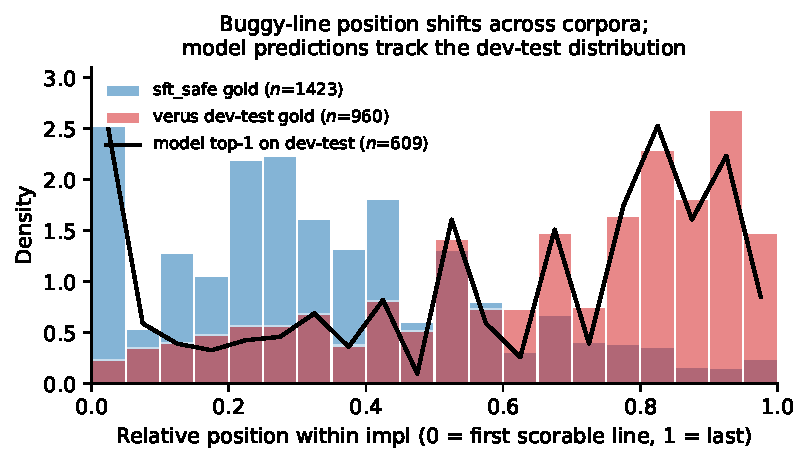
\includegraphics[width=0.80\linewidth]{fig_position_shift.pdf}
\caption{Buggy-line position distribution shifts between training
and dev-test corpora (blue: sft\_safe gold labels, median 0.31;
red: verus dev-test gold labels, median 0.74). The black line
shows our model's top-1 predictions on dev-test failures (median
0.67) --- tracking the dev-test distribution, not the training
prior. Spearman(energy, position) $= +0.03$ per impl.}
\label{fig:position-shift}
\end{figure}

\paragraph{Summary of the audit.}
The audit identifies marker leakage as the driver and rules out exact
contamination, simple line memorization, keyword-only behavior, and a
position prior. Seed variance remains a limitation
(\Cref{sec:discussion}). The script \texttt{scripts/strip\_fails\_reeval.py}
is released for re-auditing future models with the same record schema.

% =============================================================================
\section{Discussion and Limitations}
\label{sec:discussion}

\paragraph{What this paper claims.} The headline is
\emph{calibration}, not specialist superiority. The scalar-head hybrid is a
working per-line Verus fault localizer (top-3 $= 0.84$,
AUROC $= 0.78$, \Cref{tab:run10-real-bug}), and the strip-FAILS audit
pipeline is a transferable contribution. But \Cref{sec:results:cegis}
finds no closed-loop repair advantage over LLM-only or LLM-self-judged
baselines. The paper's claim is the calibration triple
(\Cref{tab:llm-zeroshot,tab:llm-discrimination,tab:cegis-3arm}) plus the
audit pipeline, not a deployable specialist recommendation.

\paragraph{What this paper does not claim.}
The architecture is a discriminative EBM in the LeCun
sense~\cite{lecun2006tutorial}; we do not claim generative density
modeling.

\paragraph{Limitations.}
\begin{enumerate}[leftmargin=*,itemsep=2pt,topsep=2pt]
\item \textbf{The Verus dev-test corpus is test-suite-authored, not
  production-derived.} Bugs are hand-written failing test cases from
  \texttt{verus-lang/verus} contributors and therefore reflect what
  Verus developers found worth testing (parser-edge cases, type
  mismatches, postcondition counter-examples), not bugs reported by
  production users. They are a substantially harder transfer target
  than the mutator-induced held set, but the gap from production-defect
  evaluation in the broader fault-localization literature should be
  kept in mind.
\item \textbf{The closed-loop CEGIS evaluation is underpowered.} We
  ran $n=100$ tractable single-buggy-line impls. The three arms
  cluster at $25$--$30\%$ repair-rate; A-vs-C has $p=0.06$ but is not
  significant. A larger evaluation ($n \ge 500$) is needed.
\item LSE-$T$ annealing during marker-leaky LSE training
  (artifact run \#7) caused observed whole-impl AUROC oscillations
  as the effective aggregator changed mid-training --- the
  ``assessment drift'' pathology of Zhang et
  al.~\cite{zhang2025lessonsprm}. The scalar-head hybrid sidesteps
  this by eliminating the LSE aggregator.
\item We did not run continued pretraining on public Verus code. A
  corpus audit of \texttt{verus-lang/verus} and
  \texttt{verus-lang/verus-tutorial} found only about 2.85MB of Rust
  files containing \texttt{verus!} macros, too small to justify a CPT
  stage under the hackathon compute budget. All domain adaptation in
  this paper therefore comes from supervised LoRA and the localization
  losses, not from unsupervised Verus-code pretraining.
\item We evaluate on Verus only. Transfer to Dafny~\cite{dafny} or
  F\textsuperscript{*} requires re-tokenization and is left
  unaddressed. A small HumanEvalPack-Rust probe~\cite{muennighoff2024octopack}
  suggests out-of-Verus deployment would need retraining or a
  verifier-agnostic per-line head.
\item Single seed. We report bootstrap CIs over the held set but do
  not retrain across seeds. A LoRA-only re-init ensemble
  (Lakshminarayanan et al.~2017) over $k=3$ seeds is the natural
  cheap variance estimate; we defer it to a longer revision.
\item Subgroup gap on \texttt{ensures}-clause failures
  (\Cref{tab:bug-type}): top-3 drops to $0.59$ on $n=22$ postcondition
  bugs. The model's per-line head can identify the line where a
  postcondition violation \emph{surfaces} less reliably than where an
  \texttt{assert} or arithmetic statement fails, likely because the
  signal for an \texttt{ensures} violation lives across the entire
  impl rather than at one local site. A global-attention head
  alongside the local sentinel head is the natural architectural
  follow-up.
\end{enumerate}

\paragraph{Implications for scalable oversight of AI-written code.}
With current frontier LLMs as proposer/rewriter, this small specialist
is not the differentiating component in our CEGIS loop. That does not
make attribution irrelevant; it shifts the question to what kind of
signal helps repair, and which actor should produce it.

\paragraph{Future work.}
The most informative follow-ups are larger-$n$ CEGIS, explicit
self-judging-loop tests, OOD Verus features, ensemble routing, a global
head for \texttt{ensures}-clause failures~\cite{ilse2018attentionmil},
and a seeded ensemble for variance estimation.

% =============================================================================
\section{Conclusion}
\label{sec:conclusion}
We built a 1.5B-parameter energy-based per-line scorer for Verus
(AUROC $=0.78$, top-1 $=0.56$, top-3 $=0.84$ on the marker-stripped
dev-test corpus) and compared it with frontier LLMs on per-line
ranking, whole-implementation discrimination, and closed-loop CEGIS
repair. The specialist beats static baselines, but frontier LLMs match
or beat it on all three comparisons; CEGIS repair-rate-at-1 is
$0.25$ specialist vs.\ $0.30$ LLM-only and $0.30$ LLM-self-judged at
$n=100$.

The durable contributions are the calibrated small-model baseline, the
line-labeled Verus corpus, the scalar-head ablation, and the strip-FAILS
audit pipeline. That audit invalidated an earlier marker-reliant result
and revealed that our fix overshot into marker-aversion, while frontier
LLMs are nearly marker-invariant. We release the corpus, model,
checkpoints, audit scripts, LLM records, and CEGIS records. The clearest
next questions are larger-$n$ CEGIS, explicit self-judging-loop tests,
OOD Verus features, and routing/ensemble approaches.

% =============================================================================
\section*{Code and Data}
\begin{itemize}[leftmargin=*,itemsep=2pt,topsep=2pt]
\item Code: \url{https://github.com/guynachshon/verificationHackathon}
\item Verus dev-test corpus: \texttt{artifacts/real\_bugs/records.jsonl}
  (1{,}492 records, 609 FAIL-with-labels, derived from
  \texttt{verus-lang/verus} test suite at HEAD).
\item Strip-FAILS audit pipeline: \texttt{scripts/strip\_fails\_reeval.py}
  (regenerates the audited corpus from the raw \texttt{// FAILS}-marked
  source for any model whose records use the same schema).
\item Headline checkpoint (scalar-head hybrid; artifact run \#10):
  \texttt{checkpoints/run10/}. Intermediate checkpoints
  (\texttt{run7\_step500}, \texttt{run9}) are released alongside for
  reproduction of the audit narrative.
\end{itemize}

\section*{LLM Usage}
We used Claude Opus to draft code, prose, and to dispatch literature-search
sub-agents. All results, numbers, and claims were independently verified
against logs and stored artifacts. The data parsers, model architecture,
losses, training loop, eval scripts, baselines, Verus dev-test scraper, and
analysis pipeline were co-authored with Claude and reviewed before commit.

% =============================================================================
\begin{thebibliography}{99}\small

\bibitem{verus2023}
A.~Lattuada, T.~Hance, C.~Cho, M.~Brun, I.~Subasinghe, Y.~Zhou, J.~Howell,
B.~Parno, C.~Hawblitzel.
\newblock Verus: Verifying Rust Programs Using Linear Ghost Types.
\newblock \emph{OOPSLA 2023}.

\bibitem{verus_training_data}
Microsoft Research.
\newblock \emph{Verus Training Data} (HuggingFace dataset
\texttt{microsoft/Verus\_Training\_Data}), 2024.

\bibitem{cegis}
A.~Solar-Lezama, L.~Tancau, R.~Bod\'{i}k, S.~Seshia, V.~Saraswat.
\newblock Combinatorial sketching for finite programs.
\newblock \emph{ASPLOS 2006}.

\bibitem{lecun2006tutorial}
Y.~LeCun, S.~Chopra, R.~Hadsell, M.~Ranzato, F.~Huang.
\newblock A tutorial on energy-based learning.
\newblock In \emph{Predicting Structured Data}, MIT Press, 2006.

\bibitem{dafny}
K.~R.~M.~Leino.
\newblock Dafny: An Automatic Program Verifier for Functional Correctness.
\newblock \emph{LPAR 2010}.

\bibitem{lightman2023letsverify}
H.~Lightman, V.~Kosaraju, Y.~Burda, H.~Edwards, B.~Baker, T.~Lee, J.~Leike,
J.~Schulman, I.~Sutskever, K.~Cobbe.
\newblock Let's Verify Step by Step.
\newblock arXiv:2305.20050, 2023.

\bibitem{wang2024mathshepherd}
P.~Wang, L.~Li, Z.~Shao, R.~X.~Xu, D.~Dai, Y.~Li, D.~Chen, Y.~Wu, Z.~Sui.
\newblock Math-Shepherd: Verify and Reinforce LLMs Step-by-Step without
Human Annotations.
\newblock \emph{ACL 2024} (arXiv:2312.08935).

\bibitem{setlur2024processadvantage}
A.~Setlur, C.~Nagpal, A.~Fisch, X.~Geng, J.~Eisenstein, R.~Agarwal,
A.~Agarwal, J.~Berant, A.~Kumar.
\newblock Rewarding Progress: Scaling Automated Process Verifiers for LLM
Reasoning.
\newblock arXiv:2410.08146, 2024.

\bibitem{cobbe2021verifiers}
K.~Cobbe, V.~Kosaraju, M.~Bavarian, M.~Chen, H.~Jun, L.~Kaiser, M.~Plappert,
J.~Tworek, J.~Hilton, R.~Nakano, C.~Hesse, J.~Schulman.
\newblock Training Verifiers to Solve Math Word Problems.
\newblock arXiv:2110.14168, 2021.

\bibitem{zhang2025lessonsprm}
Z.~Zhang, C.~Zheng, Y.~Wu, B.~Zhang, R.~Lin, B.~Yu, D.~Liu, J.~Zhou, J.~Lin.
\newblock The Lessons of Developing Process Reward Models in Mathematical
Reasoning.
\newblock arXiv:2501.07301, 2025.

\bibitem{grathwohl2020jem}
W.~Grathwohl, K.-C.~Wang, J.-H.~Jacobsen, D.~Duvenaud, M.~Norouzi, K.~Swersky.
\newblock Your Classifier is Secretly an Energy Based Model and You Should
Treat it Like One.
\newblock \emph{ICLR 2020}.

\bibitem{du2019ebm}
Y.~Du, I.~Mordatch.
\newblock Implicit Generation and Modeling with Energy Based Models.
\newblock \emph{NeurIPS 2019}.

\bibitem{bakhtin2021residual}
A.~Bakhtin, Y.~Deng, S.~Gross, M.~Ott, M.~Ranzato, A.~Szlam.
\newblock Residual Energy-Based Models for Text.
\newblock \emph{JMLR 2021} (arXiv:2004.11714).

\bibitem{abreu2007ochiai}
R.~Abreu, P.~Zoeteweij, A.~J.~C.~van Gemund.
\newblock On the Accuracy of Spectrum-based Fault Localization.
\newblock \emph{TAICPART-MUTATION 2007}.

\bibitem{just2014mutants}
R.~Just, D.~Jalali, L.~Inozemtseva, M.~D.~Ernst, R.~Holmes, G.~Fraser.
\newblock Are mutants a valid substitute for real faults in software
testing?
\newblock \emph{FSE 2014}.

\bibitem{pradel2018deepbugs}
M.~Pradel, K.~Sen.
\newblock DeepBugs: A Learning Approach to Name-based Bug Detection.
\newblock \emph{OOPSLA 2018}.

\bibitem{allamanis2021ssbd}
M.~Allamanis, H.~Jackson-Flux, M.~Brockschmidt.
\newblock Self-Supervised Bug Detection and Repair.
\newblock \emph{NeurIPS 2021}.

\bibitem{qwen25coder}
B.~Hui, J.~Yang, Z.~Cui, J.~Yang, D.~Liu, L.~Zhang, T.~Liu, J.~Zhang,
B.~Yu, K.~Lu, K.~Dang, Y.~Fan, Y.~Zhang, A.~Yang, R.~Men, F.~Huang,
B.~Zheng, Y.~Miao, S.~Quan, Y.~Feng, X.~Ren, X.~Ren, J.~Zhou, J.~Lin.
\newblock Qwen2.5-Coder Technical Report.
\newblock arXiv:2409.12186, 2024.

\bibitem{hu2021lora}
E.~J.~Hu, Y.~Shen, P.~Wallis, Z.~Allen-Zhu, Y.~Li, S.~Wang, L.~Wang,
W.~Chen.
\newblock LoRA: Low-Rank Adaptation of Large Language Models.
\newblock arXiv:2106.09685, 2021.

\bibitem{renieris2003nnqueries}
M.~Renieris, S.~P.~Reiss.
\newblock Fault Localization with Nearest Neighbor Queries.
\newblock \emph{18th IEEE International Conference on Automated Software
Engineering (ASE 2003)}, pp.~30--39, 2003.
\newblock DOI: 10.1109/ASE.2003.1240294.

\bibitem{hindle2012naturalness}
A.~Hindle, E.~T.~Barr, Z.~Su, M.~Gabel, P.~Devanbu.
\newblock On the Naturalness of Software.
\newblock \emph{34th International Conference on Software Engineering
(ICSE 2012)}, pp.~837--847, 2012.
\newblock DOI: 10.1109/ICSE.2012.6227135.

\bibitem{karampatsis2020openvocab}
R.-M.~Karampatsis, H.~Babii, R.~Robbes, C.~Sutton, A.~Janes.
\newblock Big Code $\ne$ Big Vocabulary: Open-Vocabulary Models for Source
Code.
\newblock \emph{42nd International Conference on Software Engineering
(ICSE 2020)}, pp.~1073--1085, 2020.
\newblock DOI: 10.1145/3377811.3380342.

\bibitem{anthropic2026claude47}
Anthropic.
\newblock Claude Opus 4.7 model card.
\newblock \url{https://www.anthropic.com/claude/opus}, 2026. Accessed via
OpenRouter slug \texttt{anthropic/claude-opus-4.7}.

\bibitem{openai2026gpt55}
OpenAI.
\newblock GPT-5.5 system card.
\newblock \url{https://openai.com/gpt-5.5}, 2026. Accessed via
OpenRouter slug \texttt{openai/gpt-5.5}.

\bibitem{google2026gemini35}
Google DeepMind.
\newblock Gemini 3.5 Flash technical report.
\newblock \url{https://deepmind.google/gemini-3.5}, 2026. Accessed via
OpenRouter slug \texttt{google/gemini-3.5-flash}.

\bibitem{qwen2026qwen37}
Qwen Team.
\newblock Qwen 3.7 Max model card.
\newblock \url{https://qwenlm.github.io/blog/qwen3.7-max/}, 2026. Accessed
via OpenRouter slug \texttt{qwen/qwen3.7-max}.

\bibitem{deepseek2026v4}
DeepSeek AI.
\newblock DeepSeek-V4 technical report.
\newblock \url{https://github.com/deepseek-ai/DeepSeek-V4}, 2026.
Accessed via OpenRouter slug \texttt{deepseek/deepseek-v4-pro}.

\bibitem{zhang2023selfedit}
K.~Zhang, Z.~Li, J.~Li, G.~Li, Z.~Jin.
\newblock Self-Edit: Fault-Aware Code Editor for Code Generation.
\newblock \emph{ACL 2023}.

\bibitem{delong1988comparing}
E.~R.~DeLong, D.~M.~DeLong, D.~L.~Clarke-Pearson.
\newblock Comparing the areas under two or more correlated receiver
operating characteristic curves: a nonparametric approach.
\newblock \emph{Biometrics} 44(3):837--845, 1988.

\bibitem{muennighoff2024octopack}
N.~Muennighoff, Q.~Liu, A.~Zebaze, Q.~Zheng, B.~Hui, T.~Y.~Zhuo, S.~Singh,
X.~Tang, L.~von~Werra, S.~Longpre.
\newblock OctoPack: Instruction Tuning Code Large Language Models.
\newblock \emph{ICLR 2024} (arXiv:2308.07124).

\bibitem{ilse2018attentionmil}
M.~Ilse, J.~Tomczak, M.~Welling.
\newblock Attention-based Deep Multiple Instance Learning.
\newblock \emph{ICML 2018}.

\bibitem{sun2014fastdelong}
X.~Sun, W.~Xu.
\newblock Fast Implementation of DeLong's Algorithm for Comparing the Areas
Under Correlated Receiver Operating Characteristic Curves.
\newblock \emph{IEEE Signal Processing Letters} 21(11):1389--1393, 2014.
\newblock DOI: 10.1109/LSP.2014.2337313.

\bibitem{kaushik2020counterfactual}
D.~Kaushik, E.~Hovy, Z.~C.~Lipton.
\newblock Learning the Difference that Makes a Difference with
Counterfactually-Augmented Data.
\newblock \emph{ICLR 2020}.

\bibitem{goyal2019counterfactualvqa}
Y.~Goyal, Z.~Wu, J.~Ernst, D.~Batra, D.~Parikh, S.~Lee.
\newblock Counterfactual Visual Explanations.
\newblock \emph{ICML 2019} (arXiv:1904.07451).

\bibitem{veitch2021counterfactual}
V.~Veitch, A.~D'Amour, S.~Yadlowsky, J.~Eisenstein.
\newblock Counterfactual Invariance to Spurious Correlations in Text
Classification.
\newblock \emph{NeurIPS 2021}.

\bibitem{rabin2021generalizability}
M.~R.~I.~Rabin, N.~D.~Q.~Bui, K.~Wang, Y.~Yu, L.~Jiang, M.~A.~Alipour.
\newblock On the Generalizability of Neural Program Models with Respect to
Semantic-Preserving Program Transformations.
\newblock \emph{Information and Software Technology}, 2021.

\bibitem{khosla2020supervised}
P.~Khosla, P.~Teterwak, C.~Wang, A.~Sarna, Y.~Tian, P.~Isola, A.~Maschinot,
C.~Liu, D.~Krishnan.
\newblock Supervised Contrastive Learning.
\newblock \emph{NeurIPS 2020} (arXiv:2004.11362).

\bibitem{wang2020alignment}
T.~Wang, P.~Isola.
\newblock Understanding Contrastive Representation Learning through Alignment
  and Uniformity on the Hypersphere.
\newblock \emph{ICML 2020} (arXiv:2005.10242).

\bibitem{cao2007listnet}
Z.~Cao, T.~Qin, T.-Y.~Liu, M.-F.~Tsai, H.~Li.
\newblock Learning to Rank: From Pairwise Approach to Listwise Approach
  (ListNet).
\newblock \emph{ICML 2007}.

\bibitem{schroff2015facenet}
F.~Schroff, D.~Kalenichenko, J.~Philbin.
\newblock FaceNet: A Unified Embedding for Face Recognition and Clustering.
\newblock \emph{CVPR 2015} (arXiv:1503.03832).

\bibitem{wu2017samplingmatters}
C.-Y.~Wu, R.~Manmatha, A.~J.~Smola, P.~Krähenbühl.
\newblock Sampling Matters in Deep Embedding Learning.
\newblock \emph{ICCV 2017} (arXiv:1706.07567).

\bibitem{xia2008listmle}
F.~Xia, T.-Y.~Liu, J.~Wang, W.~Zhang, H.~Li.
\newblock Listwise Approach to Learning to Rank: Theory and Algorithm
  (ListMLE).
\newblock \emph{ICML 2008}.

\bibitem{lin2017focal}
T.-Y.~Lin, P.~Goyal, R.~Girshick, K.~He, P.~Dollár.
\newblock Focal Loss for Dense Object Detection.
\newblock \emph{ICCV 2017} (arXiv:1708.02002).

\end{thebibliography}

% =============================================================================
\appendix
\section{Additional results}
\label{app:additional}

\paragraph{Eval-time aggregator sweep on Verus dev-test records.}
Same per-line energies, different reducer:
$\text{mean}{=}0.471$, $\text{max}{=}0.484$, $\text{min}{=}0.490$,
$\text{last}{=}0.517$, $\text{sum}{=}0.530$, $\text{softplus-sum}{=}0.475$,
$\text{LSE(train-time)}{=}0.487$ (\Cref{tab:agg-sweep} in main text).

\paragraph{Z-score top-$k$ aggregator (Option B$'$ from
\cite{lecun2006tutorial}-style reformulation; not headline-defensible due to
``assessment drift''):}
within-impl z-score normalize per-line energies, then mean of top-$k$.
On Verus dev-test records: $k{=}1$: $0.504$; $k{=}2$: $0.451$; $k{=}3$: $0.424$;
$k{=}5$: $0.420$. No reducer escapes the chance band; the ceiling holds.

\section{Significance tests: scalar-head hybrid vs.\ baselines}
\label{app:significance}

\Cref{tab:significance} gives paired significance tests for the scalar-head hybrid
(stripped) against the six static baselines on the Verus dev-test corpus. Top-$k$
tests are paired McNemar (exact binomial when $b_{01}+b_{10}<25$, $\chi^2$
with continuity correction otherwise). AUROC tests are paired DeLong
following Sun and Xu's fast implementation~\cite{sun2014fastdelong} of
the original procedure~\cite{delong1988comparing}. All tests use the same
$n=1{,}492$ records (or $n_{\text{labeled}}=609$ FAIL records for top-$k$)
joined by \texttt{impl\_id}; no records are excluded.

% Auto-generated by scripts/significance_tests.py
% Run #10 stripped vs trivial/zero-shot baselines on real-bug corpus.
\begin{table}[t]
\centering
\small
\caption{Paired significance tests: run \#10 (stripped) vs baselines on $n=1{,}492$ real-bug records ($n_{\text{labeled}}=609$ FAIL with line labels). Top-$k$ p-values are McNemar (paired binomial); AUROC p-values are DeLong. \textbf{Bold} = run \#10 better.}
\label{tab:significance}
\begin{tabular}{lrrrrrrr}
\toprule
Baseline & $n$ & \multicolumn{2}{c}{top-1} & \multicolumn{2}{c}{top-3} & \multicolumn{2}{c}{AUROC} \\
 & & rate & $p$ & rate & $p$ & val & $p$ \\
\midrule
random & 609 & 0.105 vs \textbf{0.560} & $<10^{-4}$ & 0.366 vs \textbf{0.839} & $<10^{-4}$ & 0.405 vs \textbf{0.778} & $<10^{-4}$ \\
length & 609 & 0.328 vs \textbf{0.560} & $<10^{-4}$ & 0.668 vs \textbf{0.839} & $<10^{-4}$ & 0.463 vs \textbf{0.778} & $<10^{-4}$ \\
keyword verus & 609 & 0.544 vs \textbf{0.560} & $0.529$ & 0.767 vs \textbf{0.839} & $<10^{-4}$ & 0.373 vs \textbf{0.778} & $<10^{-4}$ \\
keyword marker & 609 & 0.997 vs 0.560 & $<10^{-4}$ & 1.000 vs 0.839 & $<10^{-4}$ & 0.673 vs \textbf{0.778} & $0.006$ \\
qwen surprisal & 609 & 0.002 vs \textbf{0.560} & $<10^{-4}$ & 0.141 vs \textbf{0.839} & $<10^{-4}$ & 0.597 vs \textbf{0.778} & $<10^{-4}$ \\
diff sibling & 609 & 0.072 vs \textbf{0.560} & $<10^{-4}$ & 0.250 vs \textbf{0.839} & $<10^{-4}$ & 0.476 vs \textbf{0.778} & $<10^{-4}$ \\
\bottomrule
\end{tabular}
\end{table}


The marker-keyword baseline ($p=0.006$ on AUROC) shows the smallest gap
because by design it is a near-oracle for line-level localization on the
unstripped corpus---but even there, the scalar-head hybrid's impl-level discrimination
is statistically meaningfully better, and on the stripped corpus
(\Cref{sec:results:run10-baselines}) the gap widens further.

\section{Reproducibility}
\label{app:reproducibility}

All numbers in this paper tie to artifacts saved on disk in the
\texttt{artifacts/} directory of our released codebase:

\begin{itemize}[leftmargin=*,itemsep=2pt,topsep=2pt]
\item \textbf{Verus dev-test corpus}: \texttt{artifacts/real\_bugs/records.jsonl}
  (1{,}492 records, 609 line-labeled FAIL examples). Generated by
  \texttt{scripts/scrape\_verus\_real\_bugs.py} from the
  \texttt{verus-lang/verus} GitHub repository's test suite at HEAD
  (\texttt{source/rust\_verify\_test/tests/*.rs}, 132 files).
\item \textbf{Model scoring}: run \path{scripts/run_mutator_probe.sh}
  on \path{checkpoints/<run>} to produce
  \path{artifacts/real_bugs/<run>/eval_records.jsonl} for any released
  checkpoint (\texttt{run7\_step500}, \texttt{run9}, \texttt{run10}).
\item \textbf{Three-way audit}: run
  \path{scripts/strip_fails_reeval.py} and
  \path{scripts/token_mask_reeval.py}. These produce the
  \texttt{no\_surgery}, \texttt{stripped}, and
  \texttt{token\_masked} arms used in
  \Cref{tab:strip-fails-headline,tab:llm-marker-audit}.
\item \textbf{Significance + subgroups}: run
  \path{scripts/significance_and_subgroups.py} on the above eval records.
\item \textbf{Position-shift figure}: \path{scripts/figure_position_shift.py}.
\item \textbf{LLM baselines}: \path{scripts/baseline_llm_zeroshot.py}
  (ranking-prompt) and \path{scripts/baseline_llm_discrimination.py}
  (discrimination-prompt). OpenRouter slug names listed in the
  reproducibility note in \Cref{sec:results:llm-zeroshot}.
\item \textbf{CEGIS three-arm experiment}: run
  \path{scripts/cegis_demo_3arm.py} and
  \path{scripts/cegis_rerun_arm_b.py}. These produce
  \path{artifacts/cegis/3arm_results_v2.jsonl} and
  \path{summary_3arm.json}. Requires a local Verus toolchain
  binary; we used the prebuilt
  \path{verus-0.2026.05.17.e479cce-arm64-macos}.
\end{itemize}

\paragraph{Hyperparameters.}
LoRA rank 16, alpha 32, dropout 0.05; all-linear target modules
plus rank-8 \texttt{embed\_tokens}. Per-line head: MLP $1536 \to 256 \to 1$,
GELU, dropout 0.1, init-std 0.02. Optimizer AdamW ($\beta_1 {=}0.9$,
$\beta_2 {=} 0.95$), peak LR $1{\times}10^{-4}$, cosine schedule with
$3\%$ warmup decaying to $10\%$ of peak. LSE temperature linearly
annealed $1.0 \to 0.3$ across the full schedule (the source of the
assessment-drift event documented in \Cref{sec:discussion}). Loss weights:
$\lambda_{\text{spec}} = 3.0$, $\lambda_{\text{line}} = 1.0$, line-loss
margin $1.0$. Per-batch composition: at least 2 trajectory triples + 4
sft\_safe pairs. Micro-batch 16, no grad-accum, bf16 precision,
gradient checkpointing on. Max sequence length 4096. Sentinel token:
\verb+<|fim_pad|>+ (id $151662$ in Qwen2.5-Coder tokenizer).

\paragraph{Hardware.}
Single A100 SXM 80GB (RunPod community cloud, USD~\$1.39--1.49/hr).
Marker-leaky LSE (run~\#7) total wallclock: $\sim$3h to reach step 1845 before
stop-point. The step-500 checkpoint we report from required
$\sim$30 minutes of training.

\section{Marker-leak fix: from mixed-marker augmentation to scalar-head hybrid}
\label{app:marker-aug}

The strip-FAILS audit (\Cref{sec:results:strip-fails-audit})
revealed a Qwen pretraining-prior leak through \texttt{// FAILS}
comment tokens. The training corpus contains \emph{zero} such
markers, while $42.9\%$ of dev-test records do; the model inherited
the marker$\to$buggy association from pretraining. We attempted three
fixes.

\paragraph{Mixed-marker augmentation (run \#8; failed).} We injected
markers on any line and added positive distractors
(\texttt{// ok}/\texttt{// verified}), following counterfactual
augmentation work~\cite{kaushik2020counterfactual,goyal2019counterfactualvqa,veitch2021counterfactual,rabin2021generalizability}.
Held-set performance collapsed (AUROC $0.53$, top-3 $0.23$), likely
because distractors on buggy lines created within-class label noise for
the contrastive objective~\cite{khosla2020supervised,wang2020alignment}.

\paragraph{Adversarial-marker LSE (run \#9; partial fix).} We then
placed \texttt{// FAILS}-family markers only on random non-buggy lines.
This shrank the marker-leak top-3 gap from $33$pp to $4$pp, but
whole-impl AUROC inverted to $0.40$ while top-3 reached $0.87$. The
LSE aggregator inherited an implementation-level bias that simple
mean-subtraction did not fix.

\paragraph{Scalar-head hybrid (run \#10; architectural fix).} We
therefore added a directly trained scalar attention-pool head over
$[$spec; impl$]$ hidden states, avoiding LSE aggregation, with losses
$L = \lambda_{\text{scalar}} L_{\text{impl-pair}} +
\lambda_{\text{list}} L_{\text{listwise}} +
\lambda_{\text{pair}} L_{\text{semi-hard}}$
where $L_{\text{listwise}}$ is ListNet softmax cross-entropy within
an impl~\cite{cao2007listnet} and $L_{\text{semi-hard}}$ is per-line
pairwise hinge with FaceNet-style semi-hard top-$k$
mining~\cite{schroff2015facenet,wu2017samplingmatters}. The impl-pair
loss is logistic pairwise $\text{softplus}(E^+ - E^-)$.

\paragraph{Scalar-head hybrid three-way evaluation.}

\begin{table}[htbp]
\centering
\caption{Scalar-head hybrid vs.\ baselines on the Verus dev-test corpus
($n{=}1{,}492$, $609$ FAIL with labels). Bootstrap $95\%$ CIs from
$500$ resamples. \textbf{Stripped is the canonical eval} (marker-free).}
\label{tab:run10-real-bug}
\small
\begin{tabular}{lccc}
\toprule
                                  & top-1            & top-3            & AUROC          \\
\midrule
Leaky LSE (run \#7), with markers   & 0.73             & 0.93             & 0.49           \\
Leaky LSE (run \#7), stripped      & 0.44             & 0.60             & 0.44           \\
Adv-marker LSE (run \#9), token-masked              & 0.45             & 0.80             & 0.51           \\
Adv-marker LSE (run \#9), stripped                  & 0.45             & 0.76             & 0.49           \\
\midrule
Scalar-head hybrid (run \#10), token-masked             & 0.064            & 0.388            & \textbf{0.782} \\
\textbf{Scalar-head hybrid (run \#10), stripped}        & \textbf{0.560}   & \textbf{0.839}   & \textbf{0.778} \\
Scalar-head hybrid (run \#10), no-surgery               & 0.038            & 0.238            & \textbf{0.842} \\
\bottomrule
\end{tabular}
\end{table}

\textbf{Reading.} The scalar-head hybrid is the first checkpoint in the
sweep where AUROC and top-$3$ are both above chance. Its stripped result
is the canonical leak-free metric. With markers retained, however,
top-$1$ collapses to $0.038$--$0.064$: adversarial marker training
over-corrected into marker-aversion, so the with-marker arm is reported
only for transparency.

\paragraph{Ablation: what fixed AUROC.}
We trained four single-component ablations: no scalar head (A1), no
listwise loss (A2), no semi-hard mining (A3), and hinge instead of
logistic impl-pair loss (A4). All use the same data and dev-test scorer.

\begin{table}[htbp]
\centering
\small
\caption{Single-knob ablations of the scalar-head hybrid on the marker-stripped Verus dev-test
corpus ($n{=}1{,}492$). Attribution order:
\textbf{scalar head $\gg$ listwise $>$ semi-hard mining $\gg$ logistic loss}.
The scalar attention-pool head is the load-bearing architectural change;
removing the listwise or semi-hard component degrades AUROC substantially
but leaves top-$k$ recall comparatively intact; the logistic-vs-hinge
choice is within-noise.}
\label{tab:run10-ablation}
\begin{tabular}{lccc}
\toprule
                                     & AUROC          & top-1           & top-3           \\
\midrule
Scalar-head hybrid (run \#10; reference)        & \textbf{0.778} & \textbf{0.560}  & \textbf{0.839}  \\
\textbf{No scalar head (A1; LSE)}     & 0.455          & 0.516           & 0.819           \\
\textbf{No listwise (A2)}              & 0.592          & 0.598           & 0.836           \\
\textbf{No semi-hard mining (A3)}      & 0.663          & 0.547           & 0.790           \\
\textbf{Hinge instead of logistic (A4)}& 0.784          & 0.522           & 0.847           \\
\bottomrule
\end{tabular}
\end{table}

\textbf{Reading.} Removing the scalar head collapses AUROC from $0.78$
to $0.46$, making it the load-bearing change. Removing listwise loss or
semi-hard mining hurts AUROC but less dramatically; switching logistic
back to hinge is within noise. Top-$k$ is comparatively stable because
the per-line head remains present.

\section{Strip-FAILS re-evaluation (audit pipeline)}
\label{app:strip-fails}

The audit table and its discussion are in
\Cref{sec:results:strip-fails-audit}
(\Cref{tab:strip-fails-headline}). This appendix records the released
code needed to rerun it:

\begin{itemize}[leftmargin=*,itemsep=2pt,topsep=2pt]
\item \texttt{scripts/strip\_fails\_reeval.py} --- reads
  \texttt{records.jsonl}, strips the \texttt{// FAILS} substring (and
  any trailing characters) from each line, re-tokenizes, re-scores
  with the named checkpoint, and writes \texttt{stripped.jsonl}.
\item Three-way harness: \texttt{no\_surgery}, \texttt{stripped}, and
  \texttt{token\_masked}; the token-masked arm checks whether the
  effect is tied to marker tokens rather than nearby context.
\item Mitigation: \texttt{configs/run9\_embed\_surgery.yaml} and
  \texttt{configs/run10\_hybrid.yaml} demonstrate the
  adversarial-marker-injection training fix and the architectural
  fix; both shrink the with-marker--vs--stripped top-3 gap from
  $33$pp to $\le 4$pp.
\end{itemize}

We recommend running the three-way harness before reporting transfer
numbers on comment-marked Verus tests.

\paragraph{Single-seed caveat.}
The audit numbers in \Cref{tab:strip-fails-headline} are from a
single training seed. Bootstrap CIs capture sampling variance, not
model-seed variance; a seeded LoRA ensemble is left for follow-up.

\end{document}